% ch13a Disorder: localization and exceptions, part a (书页 258-274 / 分册p001-017)
% 第13章 Disorder: localization and exceptions
\chapter{无序：局域化及其例外}

固体物理学中一个始终居于核心地位的问题是绝缘体--金属转变。这里要回答的问题是：为什么有些材料导电而另一些不导电。金属的特征是在零温下具有非零的直流电导率 $\sigma(0)$，而在绝缘体中 $\sigma(0)=0$。目前有三种标准模型可以描述这两个极端之间的转变。安德森（A1958）最先指出，来自静态但无规的势的散射可以破坏金属导电，并导致电子本征态突然的局域化。莫特（M1949）则提出，即便在 NiO 这种价带部分填充的材料中，也可以出现绝缘态。这种绝缘态起源于强电子关联，后者在费米能处打开一个能隙。能隙的闭合标志着金属态的出现，而这通常发生在中间耦合区，在该区间动能效应能够破坏势能的有序化倾向。最后，晶格周期性加倍的结构相变同样可以阻碍金属输运。尽管所有这些机制本身就具有重要的意义，本章的重点将是无序驱动的绝缘体--金属转变，即安德森转变。

我们首先回顾围绕无序诱导的局域化转变的基本物理以及若干关键争议。我们要处理的两个争议是：微扰论的作用，以及电导率在安德森转变附近是否连续。为回答后一问题，我们发展局域化的标度理论。这一方法的两个关键预言是：局域化转变是连续的，并且安德森转变只存在于 $d>2$ 的情形。也就是说，在 $d=1$ 和 $d=2$，任何大小的无序都会使所有电子态局域化。最后，弱局域化分析深刻地表明，安德森转变恰恰发生在强无序极限，即微扰论失效的极限之中。因此，任何微扰论都无法用来描述无序诱导的局域化转变。尽管如此，弱局域化中的基本物理过程——时间反演的背散射——似乎正是安德森转变背后的机制。然而，即使时间反演对称性完好无损，在 $d\leq 2$ 时标准的局域化图像仍然存在重要例外。本章最后讨论全部三个已知的例子：（1）能够挫败强局域化与弱局域化两者的那一类普遍的一维模型，即无规二聚体模型（random dimer model）；（2）薄膜中的绝缘体--超导体转变；（3）新近在稀薄二维电子气中发现的导电态。

\section{局域化入门}

安德森的原始模型源于费尔（Feher）及其合作者（FFG1955）对硅中 P、As 等施主杂质的一系列电子自旋共振实验。他们注意到，每个 $^{31}\mathrm{P}$ 核上的电子自旋在从秒到分钟的时间尺度上都保持其特征频率。然而，一个简单的黄金定则计算（与近藤问题中所作的计算属同一类型，只是此处只需保留 $O(J^{2})$ 项）预言，与其他杂质相互作用所导致的预期寿命应在 0.1 s 到 $10^{-6}$ s 之间（A1958）。费尔实验中局域自旋包的持续存在表明，$^{31}\mathrm{P}$ 杂质自旋之间不存在自旋扩散。由于宿主硅在其他方面极为纯净，安德森把自旋扩散的缺失追溯到掺杂杂质的无规分布所引起的无序。为捕捉无规势存在下量子力学输运的精髓，安德森提出了紧束缚模型
\begin{equation*}
H=\sum_{n}\epsilon_{n}a_{n}^{\dagger}a_{n}+V\sum_{n,m}a_{n}^{\dagger}a_{m}\tag{13.1}
\end{equation*}
用以描述杂质带中的导电，其中一个轨道和单个格点能量 $\epsilon_{n}$ 被随机地赋予各格点。一个恒定的最近邻矩阵元 $V$ 介导最近邻格点之间的输运。在式 (13.1) 中，$a_{n}^{\dagger}$（$a_{n}$）在格点 $n$ 上产生（湮灭）一个电子。一般地，$V$ 依赖于距离，例如在自旋扩散问题中，偶极相互作用给出的矩阵元按 $V\propto 1/r^{3}$ 衰减。不过，在矩阵元中纳入无序并不会定性地改变输运问题的性质。

式 (13.1) 中的格点无序紧束缚模型描述一个局域化--退局域化转变，通过考虑两个简单极限即可看出。我们先假定格点能量取自宽度为 $W$ 的均匀分布。当 $W=0$ 时，体系是有序的，因为所有格点具有相同的能量。所得本征态是退局域化的布洛赫态，在样品尺寸范围内不受散射。这一区域的输运是弹道式的。而在 $V=0$ 的极限下，格点之间互不相连，输运停止，也就是说，所得本征态是局域化的。因此，安德森模型所描述的局域化--退局域化转变至少部分地由比值 $V/W$ 支配。凭物理直觉，人们很想论证：在所有情形下，逐渐增大比值 $V/W$ 都会导致极端局域极限（$V=0$）与弹道区（$V\gg W$）之间的光滑插值。我们如今从局域化标度理论、以及从莫特与图斯（Twose）（MT1961）和博兰（Borland）（B1963）的早期工作得知，事实并非如此。对 $d\leq 2$，现在已经充分确立（某些特殊的一维情形除外（DWP1990））：无穷小量的无序就排除了扩展态的存在。也就是说，对 $d=1,2$，弹道区与局域区之间的光滑插值并不发生。在三维，当 $W/V$ 超过某个临界值 $(W/V)_{\mathrm{c}}$ 时，扩展态无法形成。当 $W/V<(W/V)_{\mathrm{c}}$ 时，扩展态与局域态在能带中共存，但被一个如今称为迁移率边（mobility edge）的能量 $E_{\mathrm{c}}$ 分隔开来：若粒子的能量 $E$ 超过 $E_{\mathrm{c}}$，粒子就是扩展的；在相反的区域 $E<E_{\mathrm{c}}$，则发生局域化。

\begin{figure}[H]\centering
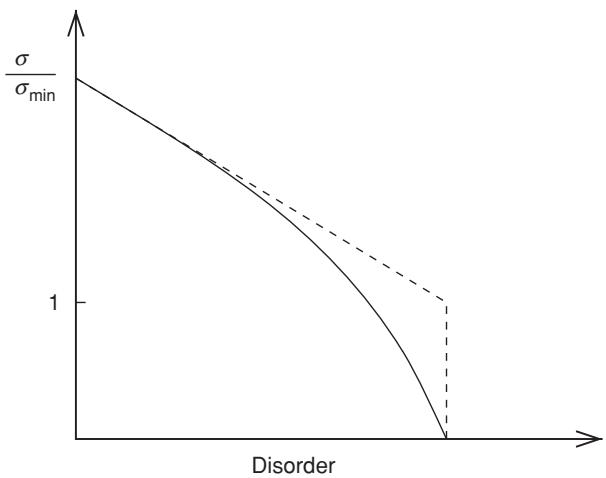
\includegraphics[width=0.55\textwidth]{figs/ch13/fig_13.1.jpg}
\caption*{图 13.1\quad 安德森转变中迁移率边附近电导率行为的两种可能性。虚线表示莫特的最小金属电导率假设；实线则描绘安德森转变处电导率的连续下降。实验上观测到的是后者，这也是局域化标度理论的预言。}\label{fig:auto:13.1}
\end{figure}

在局域化转变的语境中自然产生的一个问题是：迁移率边附近电导率会发生什么？有两种可能：要么电导率从金属一侧逼近迁移率边时连续地趋于零；要么如莫特（M1972）所提出的，$\sigma$ 先降到某个最小值，然后不连续地骤降到零。这两种可能性都绘于图 13.1 中。莫特最小电导已被证明是针对局域化转变提出的观念中最具争议然而却是错误的观念之一。不过，只要把 Drude 直流电导率改写成
\begin{equation*}
\sigma(0)=\frac{e^{2}n_{\mathrm{e}}\tau}{m}\approx\left(\frac{e^{2}}{\hbar}\right)\frac{\mathsf{a}^{2-d}}{\pi}\frac{\ell}{\mathsf{a}}=\sigma_{0}\frac{\ell}{\mathsf{a}}\text{，}\tag{13.2}
\end{equation*}
即用平均自由程 $\ell=v_{\mathrm{F}}\tau$ 来表示，这一想法的直观吸引力便立刻显现出来。我们把 $d$ 维体系的电子密度近似为 $n_{\mathrm{e}}=\mathsf{a}^{-d}$，其中 $\mathsf{a}$ 是晶格常数。无序通过比值 $\ell/\mathsf{a}$ 进入。显然，若 $\ell$ 有一个最小值，那么 $\sigma(0)$ 也会有。在玻尔兹曼输运理论中，$\ell$ 不能小于晶格常数。因此莫特（M1949）假定必须存在形如 $\sigma_{\mathrm{min}}=b\sigma_{0}$ 的最小金属电导率。常数 $\sigma_{0}$ 是普适的，而 $b$ 一般取在 0.08 与 0.3 之间。最小金属电导率假设认为，$\sigma(0)$ 应当随 $\ell$ 减小，因而一旦 $\ell=\mathsf{a}$ 就应当骤降到零，如图 13.1 所绘。实验上这一预言并未得到证实：如今已有许多在局域化转变附近测得低于 $\sigma_{\mathrm{min}}$ 的电导率的例子。此外，局域化标度理论预言转变是连续的。这两个结果都彻底否定了 $\sigma_{\mathrm{min}}$ 假设。我们将会看到，安德森转变无法在玻尔兹曼输运理论的框架内描述，因此玻尔兹曼理论对平均自由程所施加的最小值是不正确的。

\section{回归概率：局域化判据}

安德森局域化理论至少应当提供一种区分局域态与扩展态的准确方法。为此，我们关注回归概率（return probability）。考虑在 $t=0$ 时刻把一个粒子放置在格点无序的 $d$ 维晶格的原点上。由于跳跃项的存在，粒子有离开原点的有限概率。那么我们可以问：当 $t\to\infty$ 时，原点处是否还残留任何概率？如果当 $t\to\infty$ 时原点处的概率保持非零，那么粒子就有有限的概率返回原点，因而它是局域化的。反之，如果原点处的概率衰减到零，粒子将可能出现在整个晶格各处，因而是退局域化的。格点回归概率是局域化问题中的关键量（A1958；AAT1973）。此外，正是时间反演闭合路径之间的相位关系导致了弱局域化。

在式 (13.1) 模型的语境中，我们定义 $c_{n}(t)$ 为电子在时刻 $t$ 处于格点 $n$ 的概率幅。长时间下的回归概率由格点概率幅的平方决定，即 $\lim_{t\to\infty}|c_{n}(t)|^{2}$。为得到这个量，我们关注海森堡运动方程
\begin{equation*}
\mathrm{i}\hbar\dot{c}_{n}(t)=\epsilon_{n}c_{n}+\sum_{m}V_{nm}c_{m}\text{，}\tag{13.3}
\end{equation*}
其中 $V_{nm}$ 在格点 $n$ 与 $m$ 互为最近邻时等于 $V$，否则为零。由这一方程清楚地看到：没有跳跃项时，格点概率不会偏离其初值演化，因此初始局域的分布将保持局域。令人惊讶的是，即使跳跃项非零，概率幅也存在局域解。局域化判据可以如下建立。我们先对运动方程作拉普拉斯变换
\begin{equation*}
c_{n}(E)=\frac{\mathrm{i}\hbar c_{n}(t=0)}{\mathrm{i}E-\epsilon_{n}}+\sum_{m\neq n}\frac{V_{nm}c_{m}(E)}{\mathrm{i}E-\epsilon_{n}}\tag{13.4}
\end{equation*}
其定义为
\begin{equation*}
c_{n}(E)=\int_{0}^{\infty}\mathrm{e}^{-Et/\hbar}c_{n}(t)\,\mathrm{d}t\text{，}\tag{13.5}
\end{equation*}
其中 $E$ 是具有能量量纲的一般复变量。我们考虑局域的初始条件 $c_{n}(t=0)=\delta_{n0}$。拉普拉斯变换后的方程最好用迭代法求解，得到
\begin{equation*}
c_{0}(E)=\frac{\mathrm{i}\hbar}{(\mathrm{i}E-\epsilon_{0})}+\sum_{l\neq 0}\frac{V_{0l}V_{l0}}{(\mathrm{i}E-\epsilon_{0})(\mathrm{i}E-\epsilon_{l})}+\cdots\tag{13.6}
\end{equation*}
这就是原点处格点概率幅的方程。由于初始条件是局域的，$V$ 的线性项为零。由于限制 $l\neq 0$，该级数的第 $n$ 项代表从原点出发、经 $n$ 步又回到原点的自回避随机行走：除原点外没有任何格点被访问两次。我们通过为格点 $n$ 定义自能 $S_{n}(E)$ 来对式 (13.6) 的级数求和，使得
\begin{equation*}
c_{n}(E)=\frac{\mathrm{i}\hbar}{\mathrm{i}E-\epsilon_{n}-S_{n}(E)}\text{。}\tag{13.7}
\end{equation*}
所有长度的无规行走都被求和进格点自能。长时间（$E\to 0$）下的局域化问题现在取决于自能。

格点概率幅与我们原哈密顿量的精确格林函数的对角元之间存在紧密的联系。作为预解式（resolvent），格林函数 $G(E)=(E-H)^{-1}$ 包含式 (13.1) 精确本征态的全部信息。单粒子格林函数的矩阵元满足
\begin{equation*}
(E-\epsilon_{n})G_{nm}(E)=\delta_{nm}+\sum_{n\neq l}V_{nl}G_{lm}(E)\text{。}\tag{13.8}
\end{equation*}
式 (13.8) 的形式富有启发性，主要有两个原因。第一，由于紧束缚态构成原子基组，格林函数的第 $m$ 个本征态可以十分一般地写成这些态的叠加
\begin{equation*}
|\phi_{m}\rangle=\sum_{n}c_{nm}|n\rangle\tag{13.9}
\end{equation*}
系数 $c_{nm}$ 决定第 $m$ 个本征态与格点 $n$ 交叠的幅度。若没有式 (13.8) 中的第二项，格林函数的奇点就是能量 $E=\epsilon_{m}$ 处的简单极点，而精确本征态退化为 $|\phi_{m}\rangle=|m\rangle$。这对应于强局域区。当跳跃项存在时，关于局域态所能作出的最普遍的论断是：并非所有的 $c_{nm}$ 都非零。事实上，如果有足够多的格点幅为零，所得本征态便以指数衰减的包络 $\phi_{m}\propto\mathrm{e}^{-r/\xi_{m}}$ 为特征，其中 $\xi_{m}$ 是该本征态的局域化长度（空间延展尺度）。一维无规二元合金中指数局域态的一个例子示于图 13.2。

其次，格林函数对角元按 $V$ 的幂次的展开
\begin{align*}
G_{nn}(E)&=\frac{1}{(E-\epsilon_{n})}+\sum_{l\neq n}\frac{V_{nl}V_{ln}}{(E-\epsilon_{n})(E-\epsilon_{l})}+\cdots\\
&=\frac{1}{E-\epsilon_{n}-S_{n}(E)}\text{，}\tag{13.10}
\end{align*}
与格点概率幅的展开完全相同\footnote{译注：原文此式交叉项印作 $V_{nl}V_{lm}$，末行分母印作 $E-E_{n}-S_{n}(E)$；按式 (13.7) 与上下文，应分别为 $V_{nl}V_{ln}$ 与 $E-\epsilon_{n}-S_{n}(E)$。}。因此，格林函数的解析性质与回归概率的命运直接相关。一般地，$E$ 可以是复的。然而，若当 $E$ 逼近实轴时 $S_{n}(E)$ 纯为实数，则 $G_{nn}(E)$ 的奇点又一次是简单极点，本征态便是局域态。只有当 $G_{nn}(E)$ 为复数，等价地，当 $E$ 逼近 $\mathrm{Re}\,E$ 轴时 $\mathrm{Im}\,S_{n}(E)$ 不为零，扩展态才会形成。也就是说，$\mathrm{Im}\,S_{n}(E)$ 的倒数决定能量为 $E$ 的态的寿命。若能量为 $E$ 的态具有有限寿命，回归概率将在长时间后消失。对安德森模型，自能 $S_{n}(E)$ 是格点能量分布的函数，因此它们本身就是无规变量。正因如此，与局域化问题直接相关的精确量是格点自能的概率分布（A1958）。不存在扩展态的标志是：格点自能的概率分布沿实 $E$ 轴的所有能量处均为零。临界值 $(W/V)_{\mathrm{c}}$ 决定使安德森转变得以发生所需要的无序量。

\begin{figure}[H]\centering
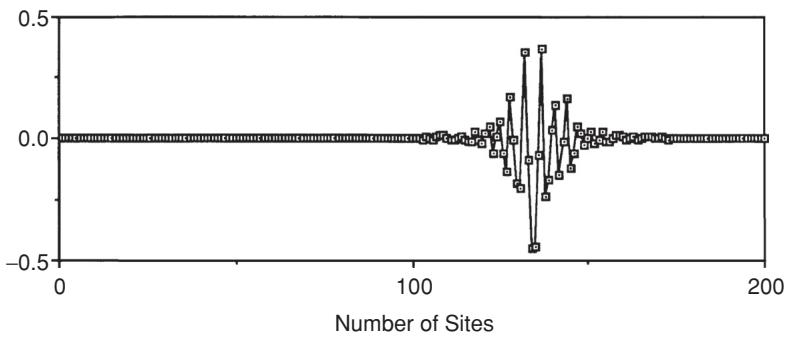
\includegraphics[width=0.62\textwidth]{figs/ch13/fig_13.2.jpg}
\caption*{图 13.2\quad 无规二元合金中一个典型本征态的实部。}\label{fig:auto:13.2}
\end{figure}

\begin{figure}[H]\centering
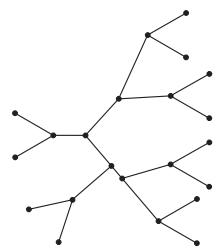
\includegraphics[width=0.35\textwidth]{figs/ch13/fig_13.3.jpg}
\caption*{图 13.3\quad 连通度 $K=3$ 的凯莱树（Cayley tree）。}\label{fig:auto:13.3}
\end{figure}

对局域化问题的格林函数分析而言，主要障碍在于格点自能的计算。自能需要对所有返回到给定格点的自回避行走进行枚举。因此，在缺乏闭合回路的晶格（例如凯莱树）上，格点自能可以精确计算。一个典型的凯莱树绘于图 13.3。在自能概率分布的分析中采用的另一个简化是忽略自能的实部。正如我们在第 7 章局域磁矩模型的语境中所证明的，只有当态密度剧烈涨落时，自能实部的贡献才是显著的。对局域化问题，计入自能实部会压低局域化转变所需的临界无序量。忽略自能实部时对安德森转变的分析（AAT1973）给出
\begin{equation*}
(W/2V)_{\mathrm{c}}=4K\ln(W/2V)_{\mathrm{c}}\tag{13.11}
\end{equation*}
此即无序的上临界值，超过它便没有任何态是扩展的。人们确实作过尝试（EC1970；SE1984）把自能分析推广到超立方晶格。在这类做法中，自能通过 $M$ 步自回避行走来计算。艾科诺穆（Economou）和科恩（Cohen）（EC1970）论证，对自能中 $M$ 阶项的 $M$ 次根作稳定性分析，便可以区分局域态与扩展态：若在 $M\to\infty$ 的极限下，自能中 $O(M)$ 项的 $M$ 次根超过 1，则 $S_{n}(E)$ 的微扰展开发散，能量为 $E$ 的电子态便是扩展态。尽管这一判据不如自能虚部概率分布消失那般精确，但正如苏库利斯（Soukoulis）和艾科诺穆（SE1984）所证明的，它对方形晶格看来给出了可靠的结果。

\section{弱局域化}

为理解导致非零回归概率的基本物理，我们关注弱局域化（A1980；B1982）。弱局域化的目标是微扰地评估那些作为安德森局域化先导的散射过程的作用。考虑一群彼此无相互作用的量子力学粒子，它们在点状散射体的无规且互不关联的分布中运动。在弱无序极限下，粒子的平均自由程 $\ell$ 远大于粒子的平均间距 $\mathsf{a}\approx k_{\mathrm{F}}^{-1}$。因此在弱局域化中 $k_{\mathrm{F}}\ell\gg 1$，于是我们可以定义小参数
\begin{equation*}
\gamma=\frac{1}{\pi k_{\mathrm{F}}\ell}\ll 1\tag{13.12}
\end{equation*}
作为无序强度的量度。目标是用 $\gamma$ 建立电导率的微扰理论。为此，我们把电导率写成
\begin{equation*}
\sigma=\sigma_{0}+\delta\sigma\text{，}\quad|\delta\sigma|\ll\sigma_{0}\tag{13.13}
\end{equation*}
即标志金属区的零阶直流电导率 $\sigma_{0}$ 与一个非平凡依赖于 $\gamma$ 的修正 $\delta\sigma$ 之和。我们将在第 11 章所述的玻尔兹曼输运极限内处理 $\sigma_{0}$。在这个极限中，所有散射事件——即使涉及对同一格点的造访——都被认为是无关联的。如果存在对同一格点反复散射的内在倾向，这一近似显然是不够的。因此，与无规杂质的平均散射速率（即线性化玻尔兹曼方程中的弛豫速率）$\tau^{-1}$ 与缺陷浓度呈线性关系。于是，$\sigma_{0}$ 具有简单的 Drude 形式
\begin{equation*}
\sigma_{0}=\frac{e^{2}n_{\mathrm{e}}}{m}\tau\text{。}\tag{13.14}
\end{equation*}
在两次散射事件之间，粒子的速度是恒定的，故 $\ell=v_{\mathrm{F}}\tau$。由于 $v_{\mathrm{F}}=\hbar k_{\mathrm{F}}/m$，零阶电导率正比于 $k_{\mathrm{F}}\ell$，或者等价地，$\sigma_{0}\propto\gamma^{-1}$。

\begin{figure}[H]\centering
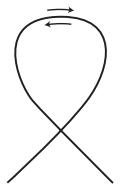
\includegraphics[width=0.20\textwidth]{figs/ch13/fig_13.4_a.jpg}\hfill
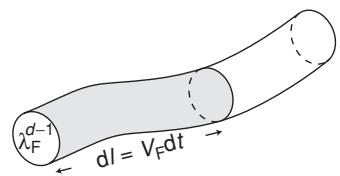
\includegraphics[width=0.45\textwidth]{figs/ch13/fig_13.4_b.jpg}
\caption*{图 13.4\quad (a) 闭合回路中的时间反演路径。(b) 量子力学粒子轨迹的体积元。横截面积为 $\lambda_{\mathrm{F}}^{d-1}$，微分长度为 $\mathrm{d}\ell=v_{\mathrm{F}}\mathrm{d}t$。}\label{fig:auto:13.4}
\end{figure}

要超出玻尔兹曼极限，我们需要考虑进入散射过程的相位关系。量子力学上，当粒子从 A 点游走到 B 点，必须对连接这两点的所有路径求和。先考虑 A 与 B 在空间上分离的情形。从 A 到 B 的一次游走的概率
\begin{equation*}
P=\sum_{i}|A_{i}|^{2}+\sum_{i,j}A_{i}A_{j}^{*}\text{，}\tag{13.15}
\end{equation*}
包含每条路径的幅 $A_{i}$ 的平方之和，以及路径之间的干涉项——式 (13.15) 中的第二项。当两个端点在空间上分离时，各路径之间没有特殊的相位关系，因而式 (13.15) 的第二项平均为零。于是玻尔兹曼处理已经足够。

然而，当 A 与 B 重合时，结果就截然不同了。考虑图 13.4(a) 所示的回路。令 $A_{1}$ 表示绕此回路顺时针路径的幅，$A_{2}$ 为时间反演路径的幅。正是在同一杂质上的重复散射中，这类回路才变得相关。我们通过变换 $\mathbf{p}\to-\mathbf{p}$ 从直接路径生成时间反演路径。由于在遍历闭合回路的过程中相位相干得以保持，$A_{1}$ 与 $A_{2}$ 相长干涉，于是可以令 $A=A_{1}=A_{2}$。因此，量子力学上遍历闭合回路的概率为 $P_{\mathrm{qm}}=|A_{1}+A_{2}|^{2}=4|A|^{2}$，而经典结果 $P_{\mathrm{cl}}=|A_{1}|^{2}+|A_{2}|^{2}=2|A|^{2}$ 要小一个因子 2，这意味着背散射效应在量子力学情形下达到最大。因此，量子力学体系中的回归概率（等价地，局域化的可能性）总是超过相应经典问题中的回归概率。这种局面的根源在于电子的波动特性。

闭合回路轨迹的贡献使电导率减小，因此 $\delta\sigma$ 以负号进入。为估计 $\delta\sigma$，我们必须确定扩散中的粒子在不损失相位相干的前提下遍历闭合回路的概率。因此，相关的时间区间从单次碰撞所需的最短时间 $\tau$ 一直延伸到相位相干丢失的最短时间 $\tau_{\phi}$。相位相干的丢失可以来自截然不同的微观现象，例如声子散射（显式的非弹性过程）以及在无磁场时不耗能量的自旋翻转散射。我们专注于计算电子遍历图 13.4(b) 所示闭合管子的概率。在这根管子中，电子具有恒定波长 $\lambda_{\mathrm{F}}=\hbar/(v_{\mathrm{F}}m)$。管子的体积随时间通过 $\mathrm{d}\ell=v_{\mathrm{F}}\mathrm{d}t$ 演化，故 $\mathrm{d}V=v_{\mathrm{F}}\lambda_{\mathrm{F}}^{d-1}\mathrm{d}t$。若允许粒子在整个空间中游荡，其均方位移将按 $D_{0}t$ 增长，这里 $D_{0}$ 是零阶扩散常数，正比于 $\sigma_{0}$，因而按 $1/\gamma$ 标度。粒子所能张开的最大"体积"元按 $V_{\mathrm{max}}\approx(D_{0}t)^{d/2}$ 标度。这一"体积"元的最大值由退相位长度 $L_{\phi}=\sqrt{D_{0}\tau_{\phi}}$ 决定。粒子出现在图 13.4(b) 所示管子中的概率
\begin{equation*}
P_{\mathrm{wl}}=\int_{\tau}^{\tau_{\phi}}\frac{\mathrm{d}V}{V_{\mathrm{max}}}=v_{\mathrm{F}}\lambda_{\mathrm{F}}^{d-1}\int_{\tau}^{\tau_{\phi}}\frac{\mathrm{d}t}{(D_{0}t)^{d/2}}\text{，}\tag{13.16}
\end{equation*}
由 $\mathrm{d}V$ 与 $V_{\mathrm{max}}$ 之比在时间区间 $[\tau,\tau_{\phi}]$ 上的积分给出。概率 $P_{\mathrm{wl}}$ 正比于 $\delta\sigma/\sigma_{0}$。完成时间积分后我们看到，弱局域化修正
\begin{equation*}
\frac{\delta\sigma}{\sigma_{0}}\approx-\gamma_{d}
\begin{cases}
\left(\dfrac{\tau_{\phi}}{\tau}\right)^{1/2}\text{，} & d=1\text{，}\\[8pt]
\hbar\ln\left(\dfrac{\tau_{\phi}}{\tau}\right)\text{，} & d=2\text{，}\\[8pt]
\hbar^{2}\left(\dfrac{\tau_{\phi}}{\tau}\right)^{-1/2}\text{，} & d=3\text{，}
\end{cases}\tag{13.17}
\end{equation*}
具有强烈的维度依赖性，其中 $\gamma_{d}=\gamma v_{\mathrm{F}}D_{0}^{-d/2}/(v_{\mathrm{F}}m)^{d-1}$。$\hbar$ 的缺席意味着：就干涉效应而言，一维弱局域化并非起源于量子力学。当然，$\hbar$ 的因子可以出现在非弹性弛豫时间之中。这类量子效应与相干背散射在性质上不同。在 $d=1$，由于只可能有前向散射与背向散射，所有路径都是闭合的。因此，就相干背散射而言，$d=1$ 时经典结果与量子结果没有差别。第二，在最低阶下，弱局域化修正线性于 $\gamma$。

若 $\tau_{\phi}$ 由声子散射或电子--电子相互作用决定，则由式 (11.96) 与式 (12.67)，$1/\tau_{\phi}\propto T^{\eta}$，其中 $\eta>0$。对声学声子，$\eta=5$（见式 (11.96)）；而对费米液体中的电子--电子散射，$\eta=2$（见式 (12.67) 及随后的讨论）。代入这一关于 $\tau_{\phi}$ 的代数形式，便得到弱局域化修正的温度依赖关系
\begin{equation*}
\frac{\delta\sigma}{\sigma_{0}}\approx-\gamma_{d}
\begin{cases}
T^{-\eta/2}\text{，} & d=1\text{，}\\[6pt]
\dfrac{\eta\hbar}{2}\ln\left(\dfrac{\hbar\tau}{k_{\mathrm{B}}T}\right)\text{，} & d=2\text{，}\\[8pt]
\hbar^{2}T^{\eta/2}\text{，} & d=3\text{。}
\end{cases}\tag{13.18}
\end{equation*}
对 $d\leq 2$，当 $T\to 0$ 时温度依赖是发散的。不过，我们这里导出的 $\delta\sigma/\sigma_{0}$ 表达式不能超过 1，这与初始假设 $|\delta\sigma|\ll\sigma_{0}$ 一致。因此，对 $d\leq 2$ 存在一个温度下限，式 (13.18) 只能在该下限之上使用。图 13.5 所示弱无序钯薄膜的电阻率测量证实了弱局域化的对数温度依赖（DO1979）。在三维，弱局域化修正随 $T\to 0$ 而消失。这反映了在三维弱无序体系中电子返回原点的概率相对较小。

\begin{figure}[H]\centering
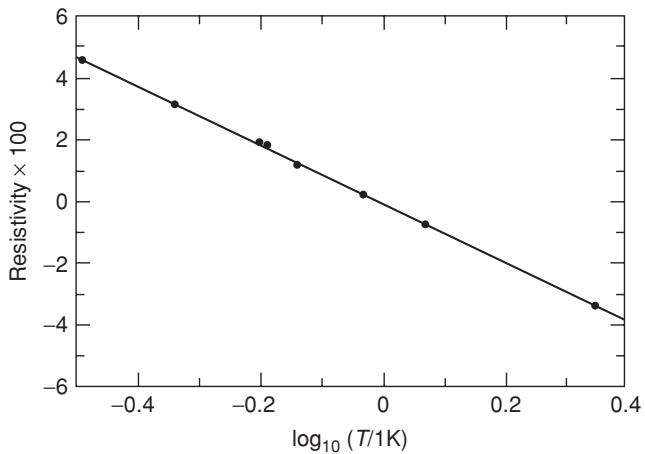
\includegraphics[width=0.55\textwidth]{figs/ch13/fig_13.5.jpg}
\caption*{图 13.5\quad Dolan 和 Osheroff（DO1979）对弱无序钯薄膜的电阻率测量。}\label{fig:auto:13.5}
\end{figure}

我们对弱局域化的分析表明，相干背散射在局域化问题中扮演着重要角色。事实上，福尔哈特（Vollhardt）和沃尔夫勒（W\"{o}lfle）（VW1980）通过把弱局域化项自洽地计入到所有阶，成功地建立了安德森局域化转变的理论，从而进一步强化了这一事实：时间反演轨迹对局域化不可或缺。由此可以合理地推断：无序体系中任何破坏时间反演对称性的外部微扰都应当摧毁局域化，从而增强电导率。例如考虑施加磁场。磁场显式地破坏了 $\mathbf{p}$ 与 $-\mathbf{p}$ 之间的对称，动量此时被 $\mathbf{p}-e\mathbf{A}/c$ 取代，其中 $\mathbf{A}$ 是矢势。沿直接路径与时间反演路径的幅分别变为 $A_{1}\to A\mathrm{e}^{\mathrm{i}\phi}$ 与 $A_{2}\to A\mathrm{e}^{-\mathrm{i}\phi}$，其中
\begin{equation*}
\phi=2\pi\frac{\Phi}{hc/e}\text{。}\tag{13.19}
\end{equation*}
磁通为 $\Phi=HR$，其中 $R$ 是图 13.4(b) 中闭合管子所围区域的面积。对扩散运动，$R$ 正比于按 $D_{0}t$ 标度的均方位移。因此，磁场存在时的回归概率
\begin{equation*}
P_{H}=4|A|^{2}\cos^{2}\left(\frac{eHD_{0}t}{\hbar c}\right)\tag{13.20}
\end{equation*}
是时间的振荡函数。相应的磁场对电导率的修正 $\Delta\sigma(H)=\delta\sigma(H)-\delta\sigma(0)$ 的计算留作课后习题（13.2）。这一修正总是正的：在强场下正比于 $H^{2}\tau_{\mathrm{in}}^{2}$，在弱场下按 $\ln(H\tau_{\mathrm{in}})$ 对数式增长。由令 $2eHD_{0}\tau_{\mathrm{in}}/\hbar c=1$ 可得从幂律交叉过渡到 $\ln H$ 的临界场。因此，交叉过渡场依赖于温度。实验上，交叉过渡场典型地为 100 G 即 10 mT 的量级。局域化对如此小的磁场的敏感性再次表明：时间反演散射是局域化转变的关键物理起源。

我们同样有能力处理的另一个类似效应，是自旋翻转散射对相位相干的破坏。自旋翻转散射削弱局域化效应，因为它提供了一个有效的振荡磁场。为量化这一效应，我们利用第 8 章中关于自旋翻转散射时间的推导。由式 (8.42)，
\begin{equation*}
1/\tau_{\mathrm{s}}=1/\tau_{\mathrm{s}}^{0}\left(1-2J_{0}N(0)\ln\frac{T_{\mathrm{F}}}{T}+\cdots\right)\text{。}\tag{13.21}
\end{equation*}
将这一结果代入式 (13.17)，便得到自旋翻转散射对 $d=2$ 样品电导率的贡献
\begin{equation*}
\delta\sigma\approx\gamma\sigma_{0}\left(\ln\frac{\tau_{\mathrm{s}}^{0}}{\tau}-N(0)J_{0}\ln\frac{T_{\mathrm{F}}}{T}\right)\tag{13.22}
\end{equation*}
由于 $J_{0}<0$，近藤对数项减小了弱局域化修正的幅度。如马丁（Martin）、万（Wan）与菲利普斯（Phillips）（MWP1997）所示，自旋翻转散射对弱局域化修正的削弱最终将导致薄膜中无序对近藤效应的压制。这一效应源于：标准近藤对数相对式 (13.21) 中的第二项以相反的符号出现。因此，若弱局域化物理占主导，无序就会压制近藤电阻率，正如在 Au(Fe) 与 Ag(Fe) 薄膜金属合金中的实验观测所示（BG1995）。由于自旋翻转散射对抗弱局域化，它常被援引来解释对标准局域化图像的偏离。例如考虑退相位时间 $\tau_{\phi}$。在电子体系中，相位相干通过与环境的耦合而丢失。与声子散射及电子--电子散射的情形一样，所有标准的退相位机制（A1980）在低温下都会关闭；因此 $\tau_{\phi}$ 在低温下应当发散。20 世纪 80 年代后期，若干实验（LG1987）报道 $\tau_{\phi}$ 在低温下饱和。磁性杂质可能起的作用使这一结果受到严重怀疑。然而，最近人们完成了更受控的实验（MJW1997），如图 13.6 所示，饱和在很宽的体系范围内持续存在，直至 $O(10\,\mathrm{mK})$ 的温度。$\tau_{\phi}$ 的表观饱和是金属物理学中真正的意外之一。事实上，如果 $\tau_{\phi}$ 随 $T\to 0$ 的饱和像当前实验似乎表明的那样被证明是一种内禀效应，那么这将对导体中量子相干所能被控制的程度施加严格的限制。截至撰写之时，对 $\tau_{\phi}$ 的饱和尚无公认的解释。

\begin{figure}[H]\centering
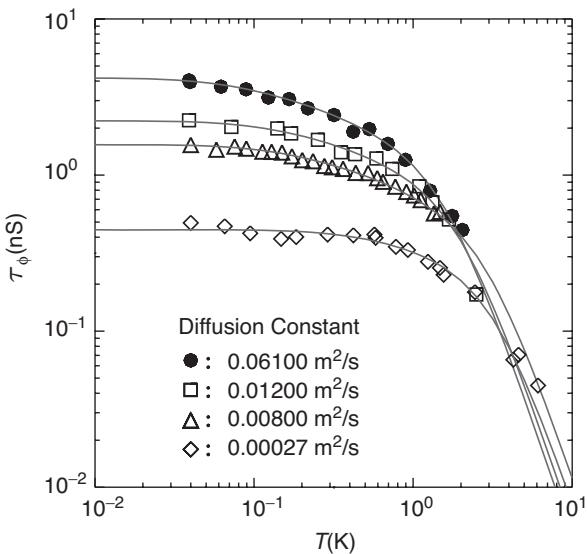
\includegraphics[width=0.55\textwidth]{figs/ch13/fig_13.6.jpg}
\caption*{图 13.6\quad 在准一维金（Au）线中观测到的电子退相位时间 $\tau_{\phi}$ 的饱和。这些样品的无序程度由经典扩散常数 $D_{0}$ 标记。无序越小，饱和时间通常越长，饱和温度越低。数据取自 P. Mohanty, E. M. Q. Jariwala, and R. A. Webb, Phys. Rev. Lett. 78, 3366 (1997)。}\label{fig:auto:13.6}
\end{figure}

\section{标度理论}

弱局域化修正强烈的维度依赖性暗示，局域化转变应当高度依赖于空间的维度。即使在较简单的问题——单个缺陷处于其余部分有序的体系中——里，维度也会介入。正如你将在习题 13.1 中证明的，放在其余部分有序的晶格中的单个缺陷，在 $d\leq 2$ 时无论其强度如何都会产生一个束缚态；对 $d>2$，缺陷强度必须超过某个临界值才能形成束缚态。尽管单缺陷结果不能直接应用于包含有限比例无格格点的无限体系，这种强烈的维度依赖性确实暗示：局域化转变应当以某种方式反映这一行为。为此，我们关注局域化的标度理论（A1979）。这一论述的关键假设是：无论维度如何，单个参数——由下式定义的无量纲电导（dimensionless conductance）
\begin{equation*}
g(L)=\frac{2\hbar}{e^{2}}G(L)\text{，}\tag{13.23}
\end{equation*}
——是样品尺寸的普适函数，并且它完全刻画了局域化转变。其中电导为 $G(L)$，$L$ 是样品的线度。对包含随机 $V$ 以及能量无序的更复杂哈密顿量，单参数标度不像对式 (13.1) 那个只含单一矩阵元 $V$ 和宽度为 $W$ 的对角无序的简单模型那样立即可见；尽管如此，它同样适用于这种情形。

另有两个关键观念锚定着局域化标度理论：（1）费米液体理论完全描述干净体系；（2）电导对体系尺寸的对数导数是电导 $g$ 的单调函数。我们将看到，这三条假设必然导致 $d\leq 2$ 时不存在载流状态，以及不存在最小金属电导率。

为发展这一标度论述，我们考虑棱长为 $L$ 的超立方晶格，并把晶格的一个原胞的尺寸放大一个因子 $p$。新晶格常数为 $L_{1}=Lp$，新原胞包含 $p^{d}$ 个原来的格点。按我们的初始假设，新原胞内的局域化性质完全由 $g(L_{1})$ 决定。经过 $m$ 次变换后，新的线度为 $L_{m}=Lp^{m}$。在这样的样品中，$g(L_{m})$ 刻画局域化转变。标度假设的一个进一步推论是：由于普适的长度依赖，所有的 $g(L_{i})$ 彼此之间必然相关联。也就是说，我们主张
\begin{equation*}
g(pL)=f(p,g(L))\text{。}\tag{13.24}
\end{equation*}
我们现在的目标是构造普适函数 $f$。如果在样品尺寸增大时各电导是相互关联的，那么本征态也是如此。而且，标度体系中的新本征态必须能够通过仅知道单个参数——无量纲电导——来构造。然而，样品尺寸增大时，能级间距 $\Delta W$ 和每个本征态的能量 $\Delta E$ 都会发生移动。因此，当取线度 $L_{1}$ 样品的本征态的线性组合来构造线度 $L_{2}$ 样品的本征态时，关键的关注量是 $\Delta E/\Delta W$（T1977）。如果一个态在初始样品尺寸内是良好局域的，把棱长从 $L$ 变到 $L_{1}$ 就不会诱发能量移动 $\Delta E$。因此，$\Delta E$ 通常通过确定本征态对边界条件的变化有多敏感来计算。计算 $\Delta E$ 时常用的一个边界效应是从周期边界条件变到反周期边界条件。由于 $\Delta E$ 对扩展态最大，而 $\Delta W$ 由态密度决定，比值 $\Delta E/\Delta W$ 应当是无量纲电导的量度。这一物理论证进一步支持了单参数标度的结论：无量纲电导必须由比值 $\Delta E/\Delta W$ 给出。

能级间的平均间距简单地由体系中粒子数的倒数给出：$\Delta W=(n_{\mathrm{e}}L^{d})^{-1}$。于是 $g(L)=n_{\mathrm{e}}L^{d}\Delta E$。那么 $\Delta E$ 呢？由量纲考虑，可以写出 $\Delta E=\hbar/\tau$，其中 $\tau$ 代表与样品中输运相关的某个物理时间。我们取 $\tau$ 为粒子从样品中心扩散到边缘所需的时间（LT1975），即 $\tau=(L/2)^{2}/D_{0}$，其中 $D_{0}$ 是扩散常数。于是 $\Delta E=2\hbar\sigma/(e^{2}n_{\mathrm{e}}L^{2})$，这里用到了爱因斯坦关系 $\sigma=2e^{2}n_{\mathrm{e}}D_{0}$。合并这些关系，我们得到
\begin{equation*}
g(L)=\frac{2\hbar}{e^{2}}\sigma L^{d-2}=\frac{2\hbar}{e^{2}}G(L)\tag{13.25}
\end{equation*}
作为局域化问题中单个参数的长度依赖。式 (13.25) 中，$G(L)=\sigma L^{d-2}$ 是直流电导。注意，这里给出的电导形式正是金属的欧姆定律。于是，单参数标度理论中的关键假设是：无量纲电导 $g$ 把棱长为 $2L$ 的样品中的本征态与线度为 $L$ 的原样品中的本征态联系起来（A1979）。

我们定义（A1979）
\begin{equation*}
\beta=\frac{\mathrm{d}\ln g(L)}{\mathrm{d}\ln L}\tag{13.26}
\end{equation*}
为 $g(L)$ 的对数导数。正如我们在近藤问题的语境中提到的，$\beta(g)$ 被称为 $\beta$ 函数（beta-function）。局域化问题的中心物理就包含在 $\beta(g)$ 之中。如果在 $L\to\infty$ 的极限下 $\beta(g)>0$，那么 $g(L)$ 必定发散。电导的发散是扩展态的标志。反之，如果当 $L\to\infty$ 时 $\beta(g)<0$，那么 $g(L)$ 在此极限下必定单调地趋于零，这时发生局域化。因此，$\beta(g)$ 的符号显然可以用来区分局域态与扩展态。援引 $\beta(g)$ 是 $g$ 或 $\ln g$ 的单调函数这一假设，必然导致 $d\leq 2$ 时不存在金属行为\footnote{译注：原文此处印作 $d>2$；按上下文（$d=1,2$ 时 $\beta(g)\leq 0$、所有态均局域化）应为 $d\leq 2$。}。我们按如下步骤进行。在弱无序极限，电导满足欧姆定律，即 $G=\sigma L^{d-2}$，因此在大电导极限下 $\beta(g)=d-2$。在强无序极限，局域化长度远小于样品尺寸（$\xi\ll L$），电导随 $L$ 指数衰减。这意味着 $\beta(g)=\ln g$ 是强无序极限（$g\ll 1$）下标度函数的形式。单调性假设保证：强无序下的形式会光滑地插值到弱无序下的渐近值 $d-2$。在弱无序区按 $1/g$ 的幂（LN1966）、以及在强局域区按 $g$ 的幂所作的微扰展开，证实了单调性假设以及这两个区域之间的连续演化。因此，对 $d=1,2$ 有 $\beta(g)\leq 0$，所有的态都是局域的。图 13.7 绘出了展示这一行为的 $\beta$ 函数。显而易见，$d=2$ 是边缘维度，在大电导极限下 $\beta(g)=0$。在 $d=3$，$\beta(g)$ 穿越 $\ln g$ 轴并渐近地趋于 1，标志着金属行为的出现。注意，$\beta$ 函数在 $d=3$ 转变附近是连续的，因而不存在最小金属电导率。

\begin{figure}[H]\centering
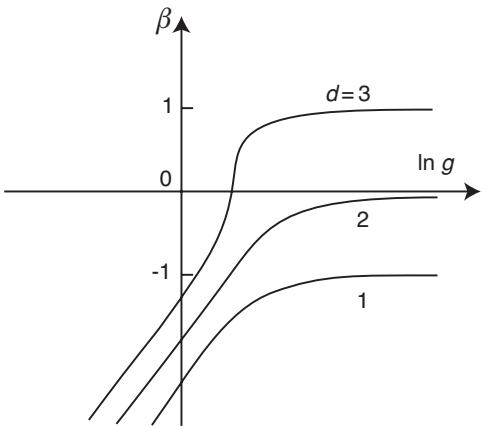
\includegraphics[width=0.50\textwidth]{figs/ch13/fig_13.7.jpg}
\caption*{图 13.7\quad 标度函数 $\beta(g)=\mathrm{d}\ln(g)/\mathrm{d}\ln L$ 作为电导 $g$ 的函数的维度依赖性。对维度 $d=1,2$，$\beta(g)$ 严格为负，且在 $d=2$ 时对大 $g$ 渐近趋于零。这表明 $d=1,2$ 不存在金属转变。在 $d=3$，$\beta(g)$ 穿越 $\beta(g)=0$ 轴并渐近地取值 $d-2$，因此标志着向金属态的转变。}\label{fig:auto:13.7}
\end{figure}

通过考虑 $\beta$ 函数在 $\beta(g_{\mathrm{c}})=0$ 附近的斜率，我们提取安德森转变附近电导的函数形式。$\beta$ 函数在 $g_{\mathrm{c}}$ 处的零点定义了临界点即不动点。在临界点 $g_{\mathrm{c}}$ 附近，我们线性化 $\beta$ 函数，使得
\begin{equation*}
\beta(g)=\frac{g-g_{\mathrm{c}}}{\nu g_{\mathrm{c}}}=\frac{\delta g}{\nu}\text{，}\tag{13.27}
\end{equation*}
其中 $\nu$ 是由斜率决定的正数。在转变点附近，电导缓慢变化。因此我们把电导的对数导数近似为 $(1/g_{\mathrm{c}})\mathrm{d}g/\mathrm{d}\ln L$。将这一结果与式 (13.27) 合并，得到
\begin{equation*}
\frac{\delta g}{\nu}=\frac{1}{g_{\mathrm{c}}}\frac{\mathrm{d}g}{\mathrm{d}\ln L}\text{，}\tag{13.28}
\end{equation*}
在区间 $[L_{0},L]$ 上积分此式，得
\begin{equation*}
\frac{L}{L_{0}}=\left(\frac{g-g_{\mathrm{c}}}{g_{0}-g_{\mathrm{c}}}\right)^{\nu}\text{，}\tag{13.29}
\end{equation*}
其中 $g_{0}=g(L_{0})$。式 (13.29) 的效用通过首先考虑 $g_{0}<g_{\mathrm{c}}$ 的局域区得以显现。引入长度尺度
\begin{equation*}
\xi=L_{0}\left(\frac{g_{\mathrm{c}}}{g_{0}-g_{\mathrm{c}}}\right)^{\nu}=L_{0}|\epsilon|^{-\nu}\tag{13.30}
\end{equation*}
之后便可以得出结论：在局域区，电导
\begin{equation*}
g=g_{\mathrm{c}}\left(1-\left(\frac{L}{\xi}\right)^{\frac{1}{\nu}}\right)\tag{13.31}
\end{equation*}
随样品长度代数式地减小。长度尺度 $\xi$ 在转变点 $g_{\mathrm{c}}$ 处发散。由于局域化长度必须在从绝缘一侧逼近不动点时发散，$\xi$ 被认定为局域化长度（这是"四人帮"（gang of four）的一个关键假设——"四人帮"是标度理论提出者们的俗称），而 $\nu$ 是其临界指数。对足够大的样品，金属一侧的电导率服从欧姆定律。然而在临界点，直流电导率以 $|\epsilon|^{s}$ 的方式消失，$s=(d-2)\nu$。我们通过如下观察来证明后一论断：标度假设保证电导在所有长度尺度上都是 $L/\xi$ 的普适函数。$L\ll\xi$ 的行为由式 (13.29) 给出。在假定欧姆定律适用的长标度下，电导必须按 $(L/\xi)^{d-2}$ 变化。由于电导率定义为 $\sigma(0)=g/L^{d-2}$，我们得到
\begin{equation*}
\sigma(0)\propto\xi^{2-d}\propto|\epsilon|^{(d-2)\nu}\text{，}\tag{13.32}
\end{equation*}
正如前文所述，电导率在临界点连续地消失，这与莫特所预言的不连续跌落相反。因此，局域化长度指数与电导率指数相互关联：$s=(d-2)\nu$（W1976）。由标度分析，$s=1$（见习题 13.5）。然而实验上（T1982），$s$ 似乎在 $1/2$ 与 1 之间变化，取决于补偿的程度。这一演化示于图 13.8。对诸如 $\mathrm{Nb}_{x}\mathrm{Si}_{1-x}$ 或补偿的 Ge:Sb 之类的材料，$s=1$；而对 Si:P 或非补偿的 Ge:Sb，$s=1/2$。在 Si:P 中，每个磷原子交出一个电子。无规势来自带电的 P 离子，因此每个散射中心都带一个电荷。在补偿的 Ge:Sb 中，加入等量的 Sb 与 B，二者随后交换一个电子。因此，补偿样品中散射体的数目超过载流子的数目。结果，无序在补偿体系中所起的作用大于在非补偿体系中的作用，因而与标度理论的符合程度得到改善。在非补偿材料中，还有自旋--轨道耦合或电子--电子排斥等附加相互作用在起作用。把这类效应计入在内会给出电导率指数 $s=1/2$（LR1985）。

弱局域化修正的对数行为也可以通过考虑二维 $\beta$ 函数的渐近形式看出。图 13.7 表明，在 $d=2$，$\beta$ 函数总是负的，并且渐近地大致按 $-1/g$ 趋于零，微扰分析也证实了这一结果。在区间 $[L_{0},L]$ 上积分这一渐近形式，便得到我们熟悉的
\begin{equation*}
g_{d=2}(L)=g(L_{0})-\ln\frac{L}{L_{0}}\tag{13.33}
\end{equation*}
电导随体系尺寸的对数式减小。与弱局域化一样，这一结果只在第二项保持小于第一项时才有效。因此存在一个长度截止，超过它微扰论便失效。

\begin{figure}[H]\centering
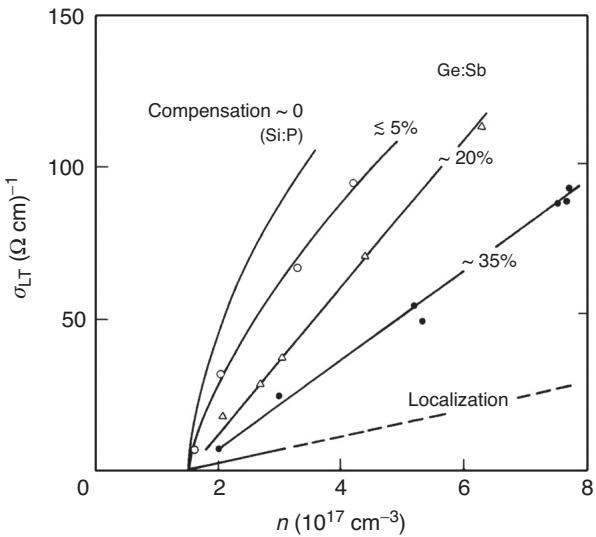
\includegraphics[width=0.55\textwidth]{figs/ch13/fig_13.8.jpg}
\caption*{图 13.8\quad 电导率指数从非补偿半导体 Si:P 中的 $s=1/2$ 向标度理论所预言的 $s=1$（虚线）演化，图中 Ge:Sb 的补偿度逐渐增大：补偿度为 0\% 时 $s=0.55$，5\% 时 $s=0.7\pm 0.2$，20\% 时 $s\approx 1$，35\% 补偿时 $s\approx 1$。$\sigma_{\mathrm{U}}$ 是低温电导率。补偿增大了无序，从而提高了安德森无序模型（标度理论预言其 $s=1$）的适用性。数据取自 G. A. Thomas et al., Phys. Rev. B 25, 4288 (1982)。}\label{fig:auto:13.8}
\end{figure}

微扰论在低温下或当 $L\to\infty$ 时的失效，标志着强局域区的开始。事实证明，上面陈述的弱局域化论证可以被修改，用以定性地处理强局域化问题。沿着上述论证的精神，我们构造粒子在时间区间 $[\tau,\tau_{\phi}]$ 内不返回原点的概率。电导率正比于这个量。粒子不返回原点的概率，等于它在每个微分时间元 $\Delta t_{i}$ 内都不返回的那些概率的乘积
\begin{equation*}
P_{\text{no return}}=\prod_{i=1}^{N}\left(1-\frac{\lambda_{\mathrm{F}}^{d-1}v_{\mathrm{F}}\Delta t_{i}}{(D_{0}t_{i})^{d/2}}\right)=\exp\left(-\sum_{i}\frac{\lambda_{\mathrm{F}}^{d-1}v_{\mathrm{F}}\Delta t_{i}}{(D_{0}t_{i})^{d/2}}\right)\tag{13.34}
\end{equation*}
把求和转换为积分留作练习（习题 13.4）。结果类似于标准的弱局域化结果，不过现在的区别在于积分位于指数上。对二维样品，我们得到电导率
\begin{equation*}
\sigma_{d=2}\approx\frac{e^{2}}{\hbar}\left(\frac{\ell}{L_{\phi}}\right)^{1/k_{\mathrm{F}}\ell\mathsf{a}}\tag{13.35}
\end{equation*}
随退相位长度代数式地标度；而对细的一维导线，电导率
\begin{equation*}
\sigma_{d=1}\approx\frac{e^{2}}{\hbar}L_{\phi}\exp\left(-\frac{1}{(k_{\mathrm{F}}\mathsf{a})^{2}}\frac{L_{\phi}}{2\ell}\right)\tag{13.36}
\end{equation*}
随相位相干长度指数式衰减。一维中电导率的指数衰减是无序局域化效应的标准特征。然而对二维，这里给出的分析不足以描述导致本征态指数局域化的相干背散射效应。

尽管局域化的标度理论非常成功，它并不构成"回归概率在 $d=1,2$ 保持有限"这一论断的数学证明。目前，对 $d$ 维无规体系中量子输运的回归概率的命运，尚无严格的数学证明。尽管如此，局域化问题的标度分析得到了更严格的理论、数值模拟以及实验（如前一段所见）的大量支持。如前几节所述，苏库利斯和艾科诺穆（SE1984）的格林函数计算证实了 $d=2$ 无序方形晶格中不存在扩展态。对局域化标度理论的进一步支持来自福尔哈特和沃尔夫勒（VW1980）的工作，他们证明标度理论的维度预言可以通过对无规势中运动的独立粒子体系的密度响应函数作自洽图形展开来重现。这项工作的另一个关键结果是：局域化问题的许多物理可以通过分析最大交叉图（maximally crossed diagrams）得到。这类图包含相干背散射的贡献。正是这些图将成为下一节的重点，因为它们包含了弱局域化物理的精髓。验证了标度预言的其他更近期的解析工作是穆塔利布（Muttalib）（M1990）的随机矩阵理论方法。基于伊姆里（Imry）（I1986）的早期工作，穆塔利布证明了如何从转移矩阵（transfer matrix）本征值的分布计算电导的最概然值。一旦假定转移矩阵本征值的分布由单个参数描述，单参数标度理论便随即得出（M1990）。尽管这一假设对强无序似乎不成立，但它在弱无序下得到数值模拟的支持（M1990）。这里只有弱无序极限是令人感兴趣的，因为正是在这个区域，单参数标度函数预言 $d=1,2$ 不存在金属转变。
